
\begin{frame}{Semana 2 (08/08/2023) - T1P1}
        $X$ e $Y$ son dos esferas de metal sin carga sobre soportes aislantes y están en contacto entre sí. Una barra R cargada positivamente se acerca a $X$ como se muestra en la figura (a).
        
        La esfera $Y$ ahora se aleja de $X$, como en la figura (b).
        
        ¿Cuáles son los estados de carga finales de $X$ e $Y$?
        
        \begin{figure}
            \centering
            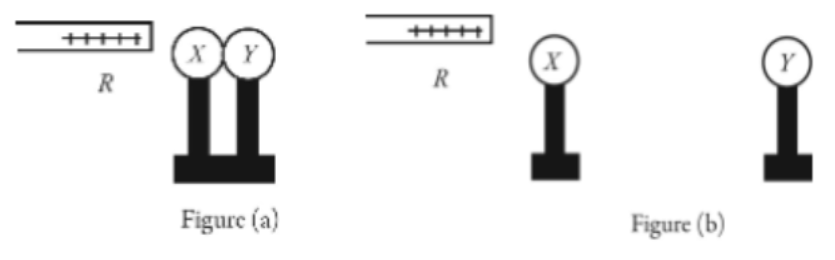
\includegraphics[scale=0.3]{figures/f1.png}
        \end{figure}
        
        \begin{columns}
        \column{0.5\textwidth}
        \begin{itemize}
            \item[A)] Tanto $X$ como $Y$ son neutros.
            \item[B)] $X$ es positivo e $Y$ es neutro.
            \item[C)] $X$ es neutro e $Y$ es positivo.
            \end{itemize}
        \column{0.5\textwidth}
        \begin{itemize}
            \item[D)] $X$ es negativo y $Y$ es positivo.
            \item[E)] Tanto $X$ como $Y$ son negativos.
        \end{itemize}
        \end{columns}
        
        
        
        \pause\bigskip\centering \textbf{Respuesta:} D.
\end{frame}

\begin{frame}{Semana 2 (08/08/2023) - T1P2}
    
    Una carga puntual positiva $Q$ está fija sobre una mesa horizontal muy grande sin fricción. Una segunda carga puntual positiva $q$ se libera desde el reposo cerca de la carga estacionaria y puede moverse libremente. ¿Qué enunciado describe mejor el movimiento de $q$ después de que se suelta?
    
    \begin{itemize}
    
    \item[A)]Su velocidad será máxima justo después de que se suelte.

    \item[B)] Su aceleración es cero justo después de que se suelta.
    
    \item[C)] A medida que se aleja más y más de $Q$, su aceleración seguirá aumentando.
    
    \item[D)] A medida que se aleja más y más de $Q$, su velocidad disminuirá.
    
    \item[E)] A medida que se aleja más y más de $Q$, su velocidad seguirá aumentando.
    \end{itemize}
    
    \pause\bigskip\centering\textbf{Respuesta:} E.
    
\end{frame}

\begin{frame}{Semana 2 (08/08/2023)- T1P3}
    
    Una bola de plástico muy pequeña cargada uniformemente está ubicada directamente encima de otra carga similar en un tubo de ensayo como se muestra en la figura. Las bolas están en equilibrio a una distancia $d$.
    
    \begin{columns}
    \column{0.5\textwidth}
     \begin{figure}
        \centering
        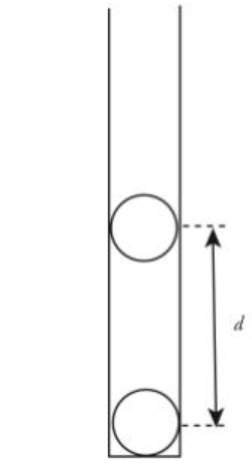
\includegraphics[scale=0.3]{figures/p2.png}
    \end{figure}
    
    \column{0.5\textwidth}

Si se duplica la carga de cada bola, la distancia entre las bolas en el tubo de ensayo sería
    
     \begin{itemize}
        \item[A)] $\sqrt{2}d$
        \item[B)] $2d$
        \item[C)] $4d$
        \item[D)] $8d$
    \end{itemize}
    
    \pause\bigskip\centering\textbf{Respuesta:} B.

    \end{columns}
    
\end{frame}

\begin{frame}{Semana 2 (08/08/2023)- T1P4}
    
    En la figura, $Q = 5.8$ nC. ¿Cuál es la magnitud de la fuerza el\'ectrica sobre la carga $Q$?
    
    \begin{figure}
        \centering
        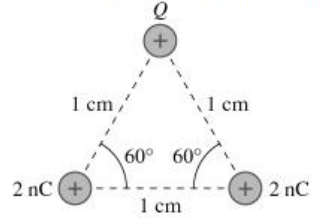
\includegraphics[scale=0.5]{figures/f3.png}
    \end{figure}
    
\end{frame}

\begin{frame}{Semana 2 (08/08/2023)- T1P5}
    Cuatro cargas puntuales negativas iguales están ubicadas en las esquinas de un cuadrado, sus posiciones en el plano $xy$ son $(1, 1)$, $(-1, 1)$, $(-1, -1)$ y $(1, -1)$. Si se posiciona una carga positiva en el punto $(1,0)$, determine la direcci\'on de la fuerza el\'ectrica que esta experimenta.
\end{frame}

\begin{frame}{Semana 2 (08/08/2023)- T1P6}
    
    Determine la magnitud y direcci\'on de la fuerza el\'ectrica que experimenta una carga puntual positiva $q$ ubicada en el punto $(L,d)$, debida a una barra delgada cargada homogéneamente con una carga $Q$ negativa y que est\'a sobre el eje $x$ en $0\leq x\leq L$.
    
\end{frame}

\begin{frame}{Semana 2 (08/08/2023)- T1P7}
    
    La figura muestra dos diminutas esferas de masa $m$ que est\'an suspendidas de dos hilos muy delgados de longitud $L$. Las esferas se repelen entre sí después de cargarse con la misma magnitud de carga $Q$ y cuelgan en reposo como se muestra en la figura. ¿Cuál es valor del ángulo $\theta$?
    
    \begin{figure}
        \centering
        \includegraphics[scale=0.4]{figures/Q1.png}
    \end{figure}
    
\end{frame}

\begin{frame}{Semana 3 (15/08/2023) - T2P1}

    La figura muestra tres cargas eléctricas etiquetadas como $Q_1$, $Q_2$, $Q_3$ y algunas líneas de campo eléctrico en la región que rodea las cargas.
    
    \begin{figure}[H]
        \centering
        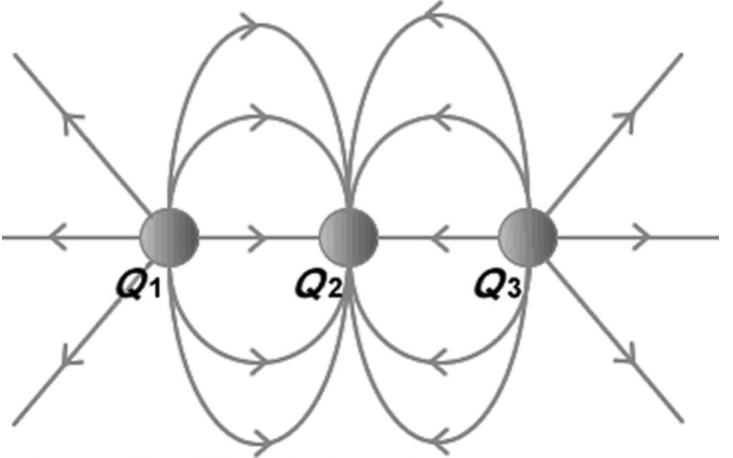
\includegraphics[scale=0.2]{figures/t2p1.png}
    \end{figure}
    
    ¿Cuáles son los signos de las tres cargas?
    
    \begin{columns}
    \column{0.5\textwidth}
    \begin{itemize}
        \item[A)] $Q_1$ es positivo, $Q_2$ es negativo y $Q_3$ es positivo.
        \item[B)] $Q_1$ es negativo, $Q_2$ es positivo y $Q_3$ es negativo.
    \end{itemize}
    \column{0.5\textwidth}
    \begin{itemize}
        \item[C)] $Q_1$ es positivo, $Q_2$ es positivo y $Q_3$ es negativo.
        \item[D)] Las tres cargas son negativas.
        \item[E)] Las tres cargas son positivas.
    \end{itemize}
    
    \end{columns}
    
    \pause\bigskip\centering\textbf{Respuesta:} A.
    
\end{frame}

\begin{frame}{Semana 3 (15/08/2023) - T2P2}

    Un electrón se mueve inicialmente hacia la derecha cuando entra en un campo eléctrico uniforme dirigido hacia arriba.
    
    \begin{figure}
        \centering
        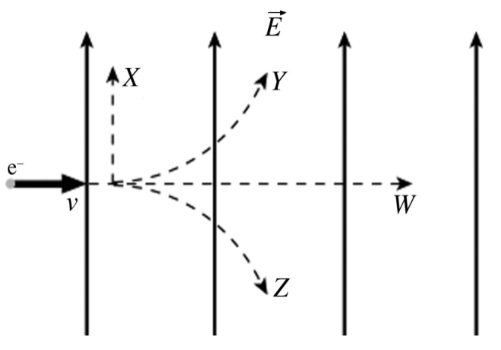
\includegraphics[scale=0.3]{figures/t2p2.png}
    \end{figure}
    
    ¿Cuál de las trayectorias mostradas seguirá el electrón?
    
    \begin{columns}
    \column{0.2\textwidth}
    
    \begin{itemize}
        \item[A)] W.
        \item[B)] X.
    \end{itemize}
    
    \column{0.2\textwidth}
    
    \begin{itemize}
        \item[C)] Y.
        \item[D)] Z.
    \end{itemize}
    
    \column{0.2\textwidth}
    \pause\centering\textbf{Respuesta:} D.
    \end{columns}
    
\end{frame}

\begin{frame}{Semana 3 (15/08/2023) - T2P3}

    Un dipolo eléctrico inicialmente estacionario de momento dipolar $\Vec{p}=\left(5.0\times10^{-10}\text{ C}\cdot\text{m }\right)\hat{\imath},$ es colocado en un campo eléctrico $\vec{E}=\left( 2.00\times10^6\text{ N/C} \right)\left(\hat{\imath}+\hat{\jmath}\right)$ ¿Cuál es la magnitud del torque máximo que el campo eléctrico ejerce sobre el dipolo?
    
\end{frame}

\begin{frame}{Semana 3 (15/08/2023) - T2P4}

    Un dipolo eléctrico consta de cargas $\pm Q$ separadas una distancia $d$. Está colocado en un campo eléctrico vertical de magnitud $E$ orientado como se muestra en la figura.
    
    \begin{columns}
    \column{0.5\textwidth}
    
    \begin{figure}
        \centering
        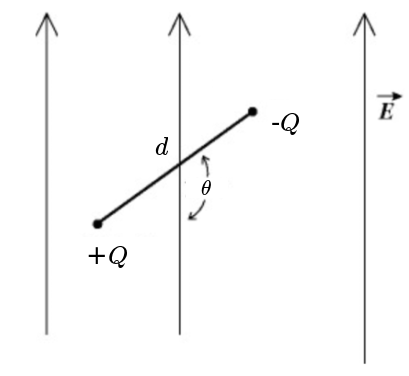
\includegraphics[scale=0.35]{figures/t2p4.png}
    \end{figure}
    
    \column{0.5\textwidth}
    
    La magnitud del torque neto que este campo ejerce sobre el dipolo est\'a dada por
    
    \begin{itemize}
        \item[A)] $QEd\sin\theta$.
        \item[B)] $\frac{QE}{2}d\cos\theta$.
        \item[C)] $QEd\cos\theta$.
        \item[D)] $\frac{QE}{2}d\sin\theta$.
    \end{itemize}
    
    \pause\bigskip\centering\textbf{Respuesta:} A.
    
    \end{columns}
    
\end{frame}

\begin{frame}{Semana 3 (15/08/2023) - T2P5}
    
    Determine la magnitud y direcci\'on de la fuerza el\'ectrica que experimenta una carga puntual positiva $q$ ubicada en el punto $(L,d)$, debida a una barra delgada cargada homogéneamente con una carga $Q$ negativa y que est\'a sobre el eje $x$ en $0\leq x\leq L$.
    
\end{frame}

\begin{frame}{Semana 3 (15/08/2023) - T2P6}

Un semicírculo de radio $a$ se encuentra en los cuadrantes primero y segundo, y con el centro de curvatura en el origen. La carga positiva $+Q$ está distribuida de manera uniforme alrededor de la mitad izquierda del semicírculo, y la carga negativa $-Q$ está distribuida de manera uniforme
alrededor de la mitad derecha del semicírculo como lo muestra la figura.

\begin{figure}
    \centering
    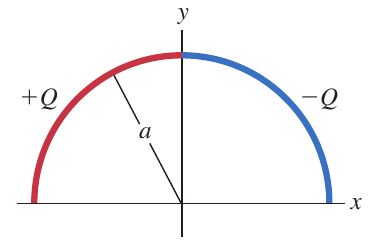
\includegraphics[scale=0.3]{figures/t2p6.png}
\end{figure}

¿Cuál es la magnitud y dirección del campo eléctrico neto en el origen generado por esta distribución de carga?
    
\end{frame}

\begin{frame}{Semana 3 (15/08/2023) - T2P7 (Bonus)}
    Considere dos alambres delgados que est\'an sobre el eje $x$. El primero se encuentra en $-d/2-L<x<-d/2$ y el segundo en $d/2<x<d/2+L$. Cada uno tiene longitud $L$ y posee carga positiva $Q$ distribuida uniformemente.
    
    \begin{itemize}
        \item[a)] Determine el campo el\'ectrico que el primer alambre genera sobre el eje $x$ positivo.
        \item[b)] Demuestre que la magnitud de la fuerza el\'ectrica que un alambre ejerce sobre el otro est\'a dada por
        
        \begin{equation}
            F=\frac{1}{4\pi\epsilon_0}\left(\frac{Q}{L}\right)^2\ln\left[\frac{\left(d+L\right)^2}{d(d+2L)}\right]
        \end{equation}
        
        \item[c)] Demuestre que si $L>>d$, entonces
        
        \begin{equation}
            F=\frac{1}{4\pi\epsilon_0}\left(\frac{Q}{d}\right)^2.
        \end{equation}
        
    \end{itemize}

\end{frame}